\begin{frame}{$\chi_b$ yields in $\chi_b \to \OneS \gamma$ decays}
  \setlength{\unitlength}{1mm}
  \centering
  \resizebox{0.65\textwidth}{!}{
  \begin{picture}(150,120)
    \put(0,0){
      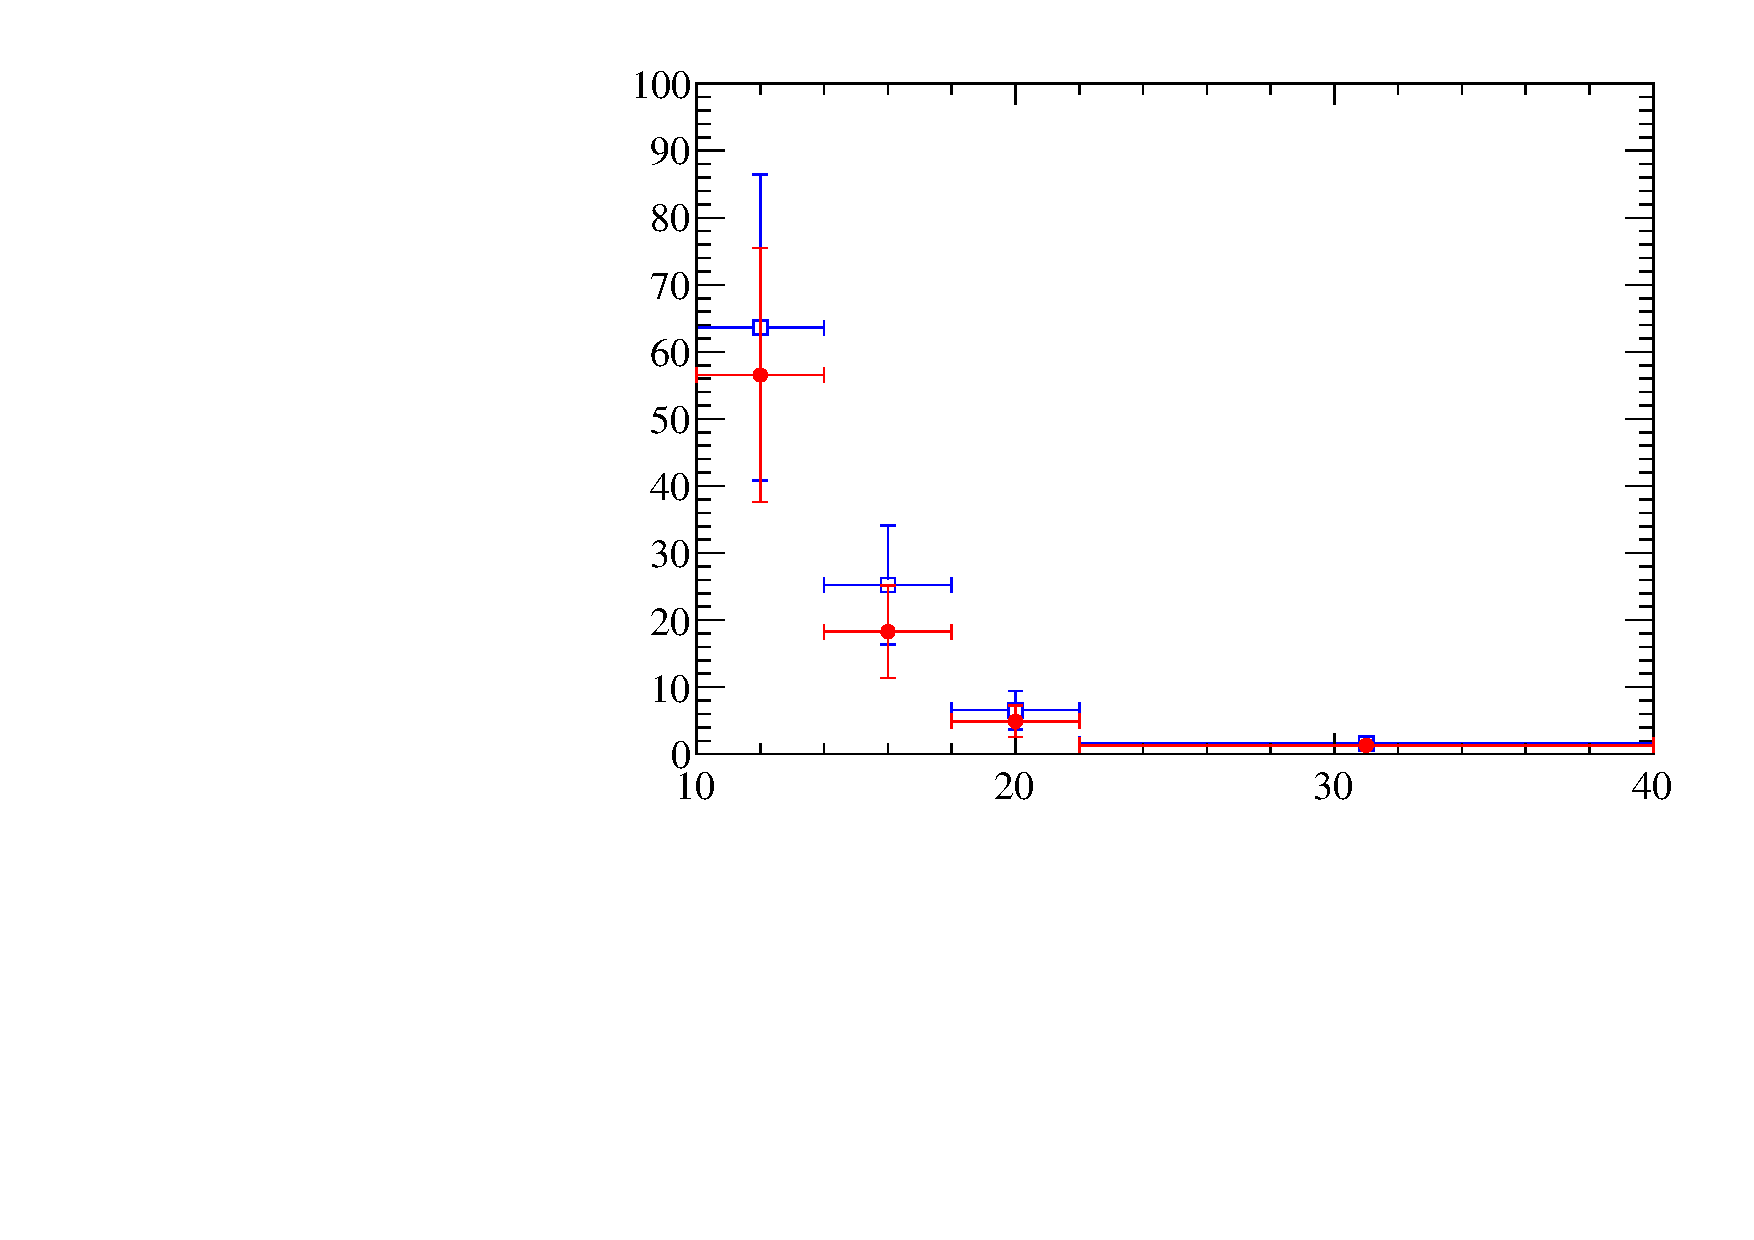
\includegraphics[width=75mm, height=60mm]{chib1s-yields/N3P_scaledbylum}
    }
    \put(0,60){
      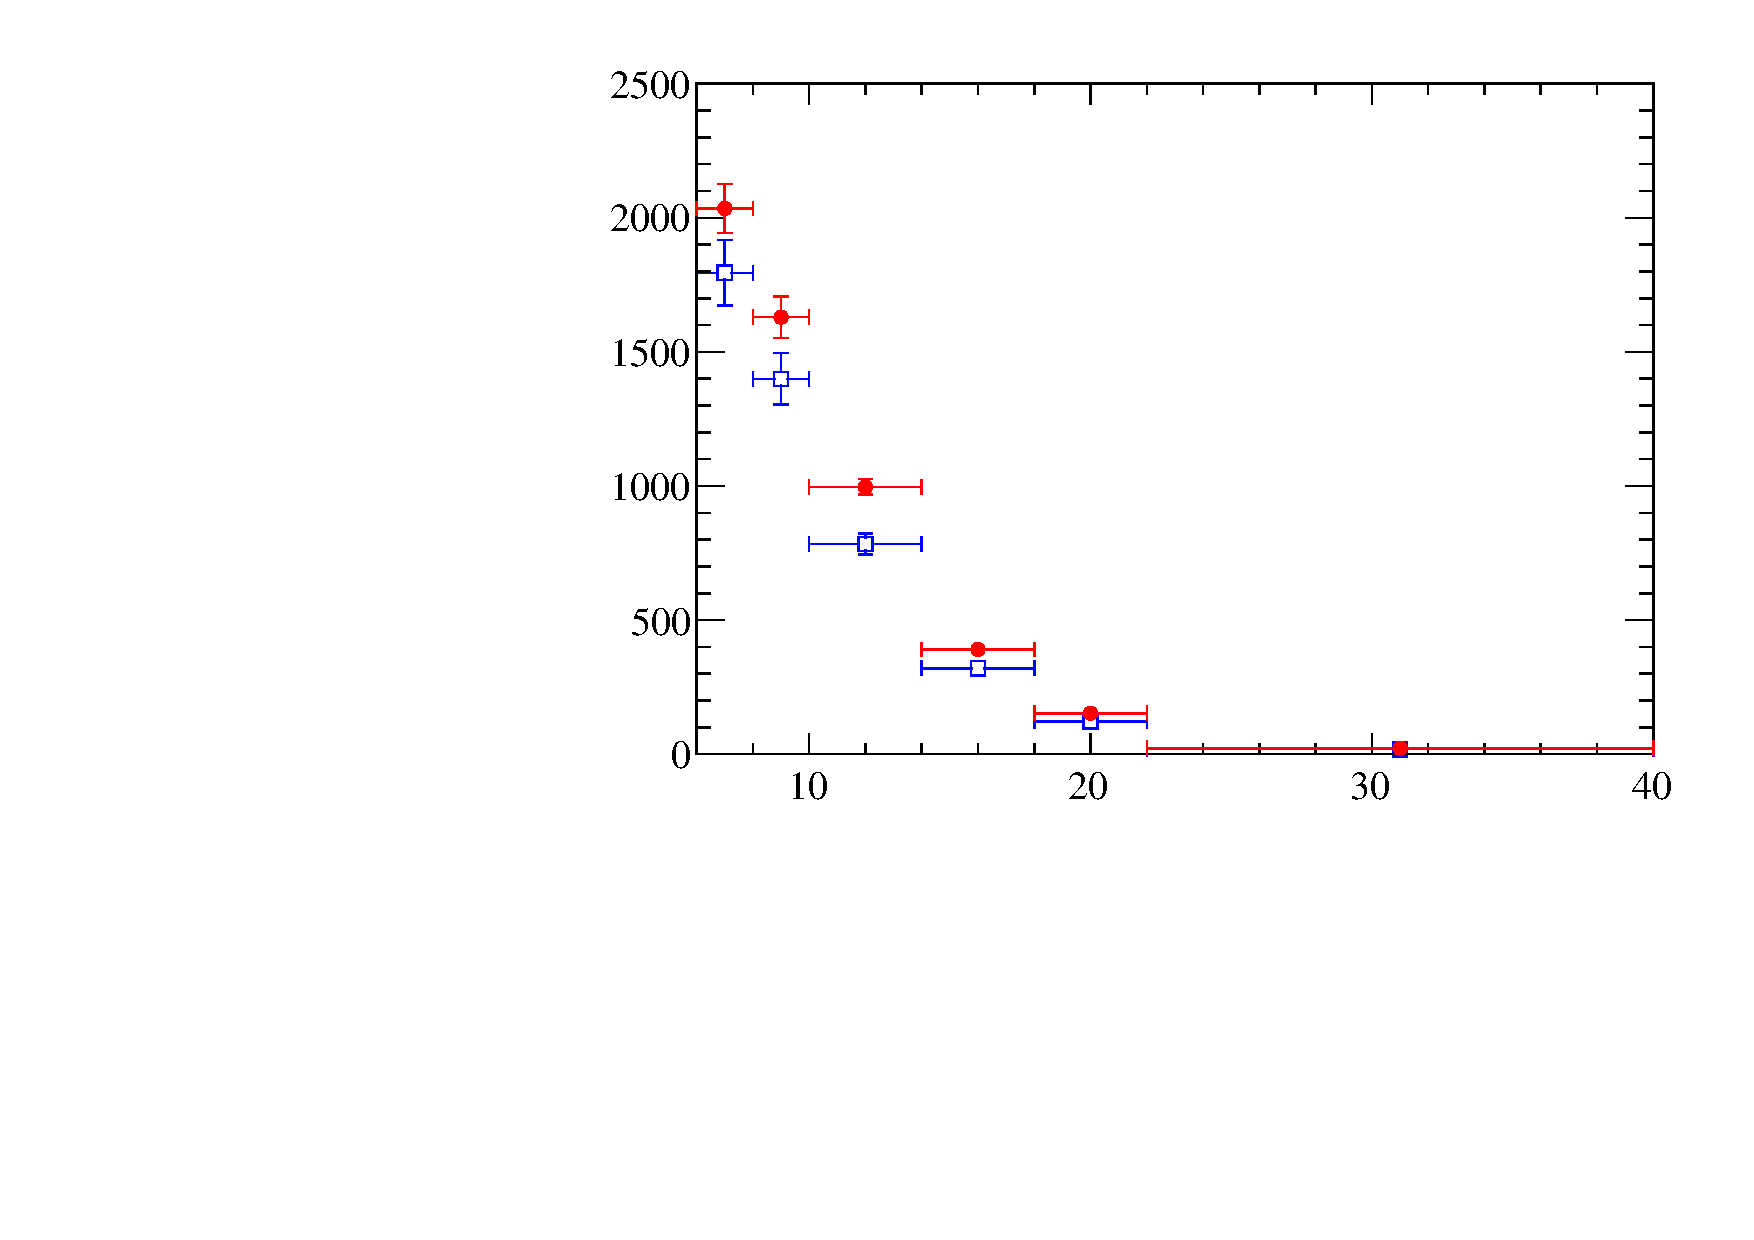
\includegraphics[width=75mm, height=60mm]{chib1s-yields/N1P_scaledbylum}
    }
    \put(75,60){
      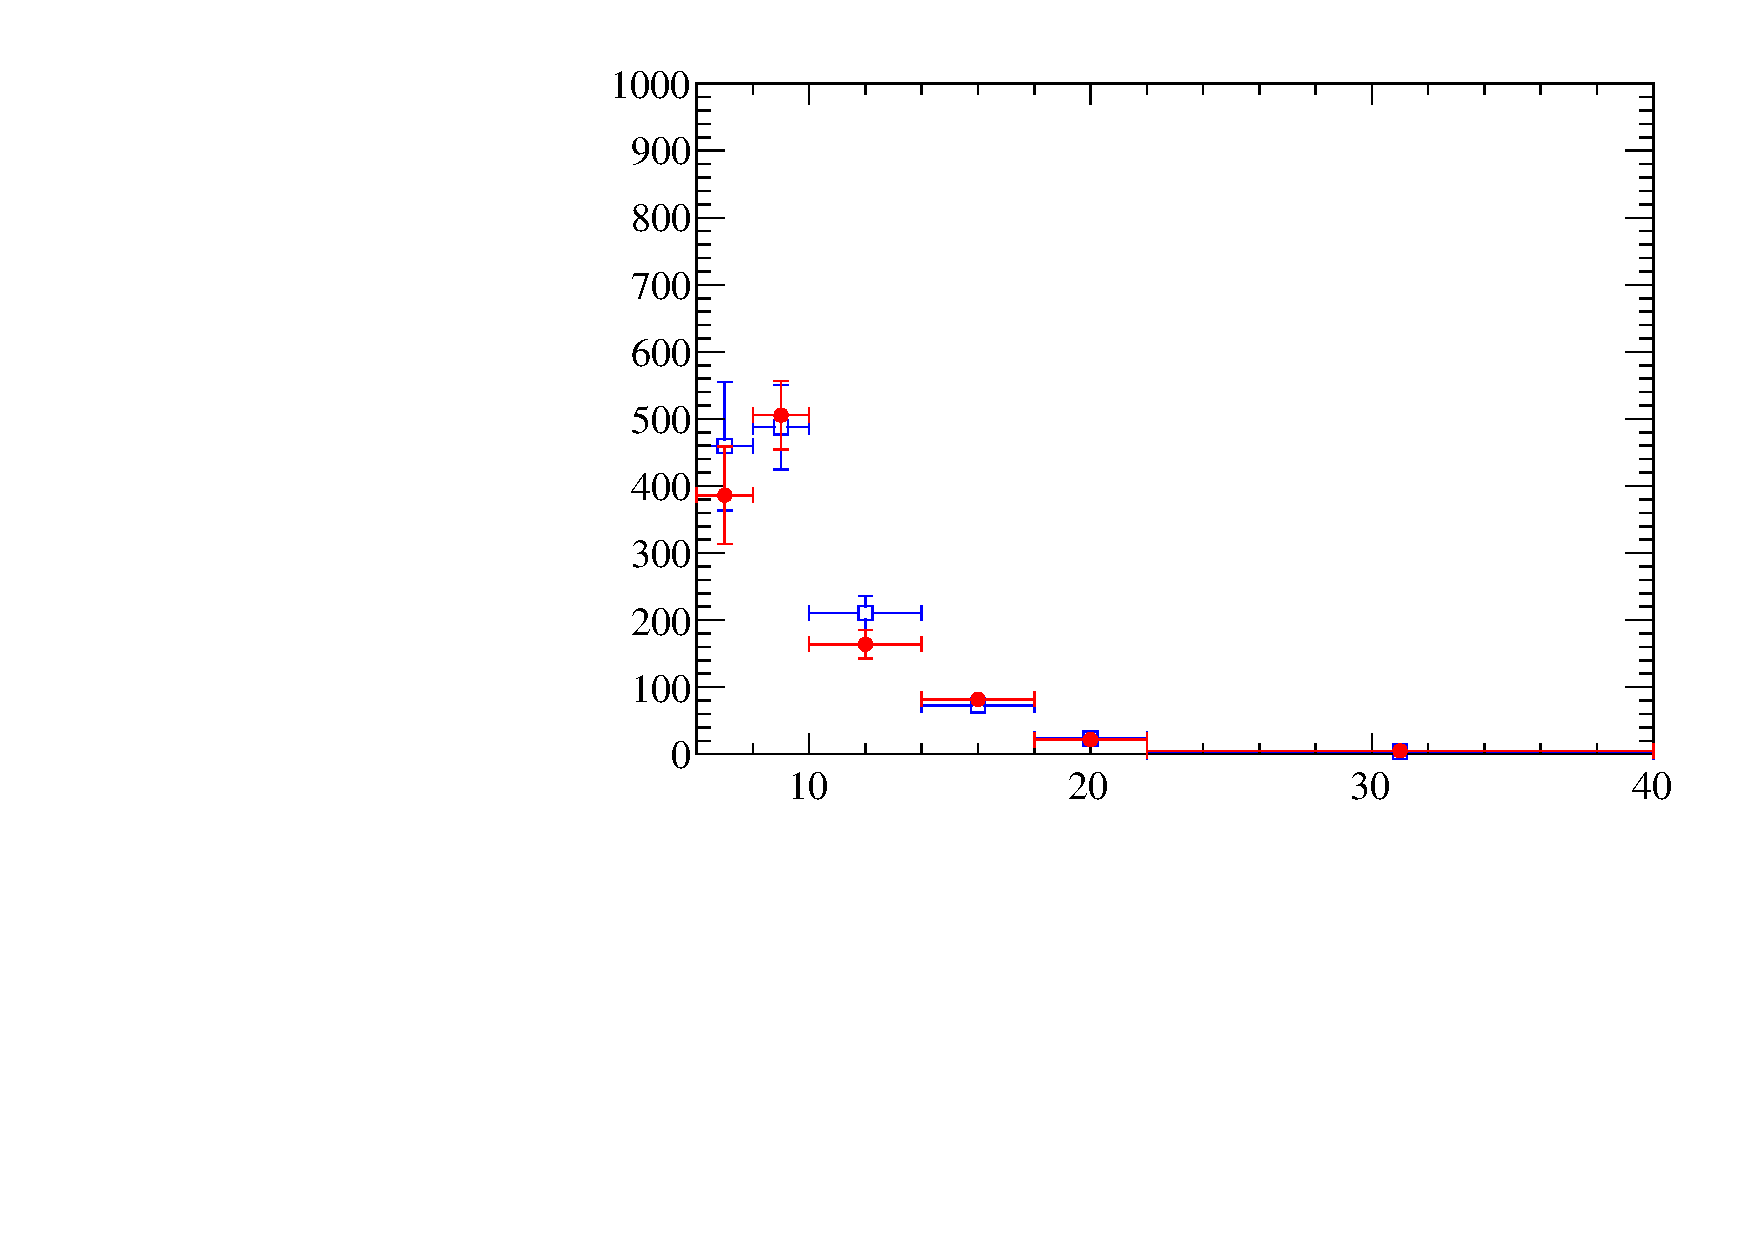
\includegraphics[width=75mm, height=60mm]{chib1s-yields/N2P_scaledbylum}
    }

    \put(2,25){\begin{sideways}Events\end{sideways}}
    \put(35,2){$p_T^{\Y1S} \left[\gevc\right]$}
    \put(55,50){$\chibThreeP$}

    \put(2,85){\begin{sideways}Events\end{sideways}}
    \put(35,62){$p_T^{\Y1S} \left[\gevc\right]$}
    \put(55,110){$\chibOneP$}

    \put(77,85){\begin{sideways}Events\end{sideways}}
    \put(110,62){$p_T^{\Y1S} \left[\gevc\right]$}
    \put(130,110){$\chibTwoP$}


    \put(50,45){\textcolor{blue}{\sqs=7\tev}}
    \put(50,40){\textcolor{red}{\sqs=8\tev}}
    \put(45,45){
      
\includegraphics[width=3mm, height=2mm]{bsf}
    }
    \put(45,40){
      
\includegraphics[width=3mm, height=2mm]{rco}
    }

    \put(50,105){\textcolor{blue}{\sqs=7\tev}}
    \put(50,100){\textcolor{red}{\sqs=8\tev}}
    \put(45,105){
      
\includegraphics[width=3mm, height=2mm]{bsf}
    }
    \put(45,100){
      
\includegraphics[width=3mm, height=2mm]{rco}
    }

    \put(125,105){\textcolor{blue}{\sqs=7\tev}}
    \put(125,100){\textcolor{red}{\sqs=8\tev}}
    \put(120,105){
      
\includegraphics[width=3mm, height=2mm]{bsf}
    }
    \put(120,100){
      
\includegraphics[width=3mm, height=2mm]{rco}
   }
  % \graphpaper[5](0,0)(75, 60)
  \end{picture}
}  
\begin{center}
Yields normalized by bin width and luminosity.
\end{center}  
\begin{block}{}
The small difference between 7 and 8\tev data is due to the production
cross-sections, which are expected to be about 10\% larger..
\end{block}
\end{frame}

